
%%%%%%%%%%%%%%%%%%%%%        PERSONNAGE AU BORD D'UNE MARE
%

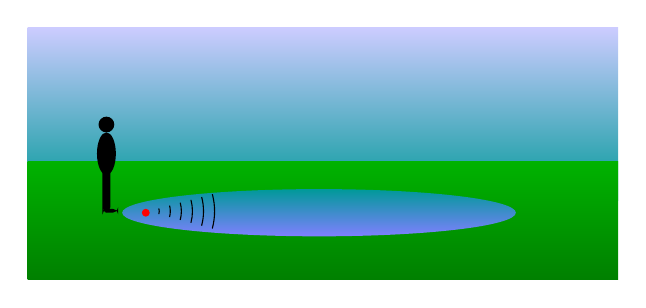
\begin{tikzpicture}
    %  Ciel
  \shade[bottom color=cyan!60!black, top color=blue!20!white] (0,0) rectangle (7.5,2.2);
    %  Sol
  \shade[bottom color=green!50!black, top color=green!70!black] (0,0.5) rectangle (7.5,-1);
    %  Mare
  \shade[bottom color=blue!50!white, top color=cyan!60!black] (3.7,-0.15) ellipse (2.5 and 0.3);
    %  Arbre
 % \pic at (2,2)    {arbre};

    %  Personnage
  \begin{scope}[xshift=1 cm,yshift=0.6 cm]
    % corps et tête
 \fill [black] (0,0)ellipse(0.12 and 0.27);
 \fill [black](0,0.37)circle(0.1);
    % jambe et pieds
 \fill [rounded corners=2pt] (0.05,-0.15)rectangle(-0.05,-0.75);
 \fill [rounded corners=2pt] (0.15,-0.7)rectangle(-0.05,-0.75);
    % bras
 %\fill [rounded corners=2pt, rotate=-15] (-0.1,0.22)rectangle(0.28,0.15);
 %\fill [rounded corners=2pt] (0.22,0.08)rectangle(0.5,0.14);
   % Balle
 \fill[red] (0.5,-0.75) circle(0.05);
  \end{scope}

    %  vague 001
\draw[decorate,decoration={expanding waves,angle=15,segment length=4pt}, rotate=7.5] (1.5,-0.33) -- (2.4,-0.45);

\end{tikzpicture}

%%%%%%%%%%%%%%%%%%%%%%%%%%%%%%%%%%%%%%%%%%%%%%%%%%%%%%%%%%%%%%%%%%%%%%%%%%%%%%%%
